\documentclass[11pt,border=2mm]{standalone}
\usepackage{csquotes}
\usepackage[backend=biber,style=numeric,sorting=none]{biblatex}

\providecommand{\FigScale}{0.69}

\providecommand{\PartGap}{2.5}

\usepackage{siunitx}
\usepackage{tikz}
\usetikzlibrary{decorations.pathmorphing,patterns}
\usetikzlibrary{shapes.geometric, arrows}
\usetikzlibrary{positioning}

\usepackage{amsmath}

\usepackage{tikz-3dplot}
\usetikzlibrary{3d}

\usepackage[siunitx,american]{circuitikz}

\usepackage{pgfplots}
\usepgfplotslibrary{units}
\usepgfplotslibrary{groupplots}
\pgfplotsset{compat=1.14}

\ctikzset{tripoles/mos style/arrows}
\begin{document}

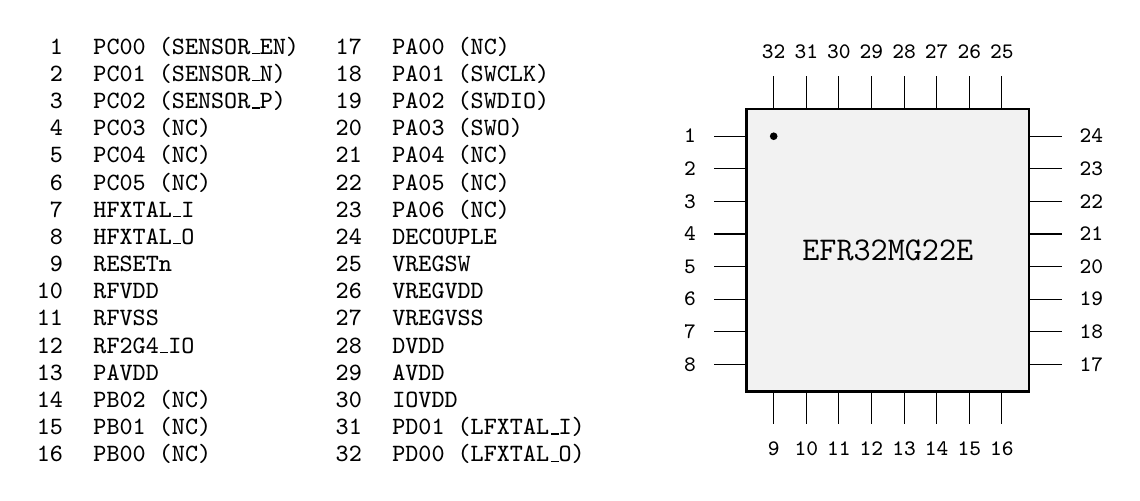
\begin{tikzpicture}[scale=\FigScale, font=\small]

\draw[thick, fill=gray!10] (-2.6,-2.6) rectangle (2.6,2.6);
\node at (0,0) {\large\texttt{EFR32MG22E}};

% Pin 1 marker
\fill (-2.1,2.1) circle (2pt);

% Left side pins (1-8, top to bottom)
\foreach \y/\n in {2.1/1, 1.5/2, 0.9/3, 0.3/4, -0.3/5, -0.9/6, -1.5/7, -2.1/8}
{
  \draw (-2.6,\y) -- (-3.2,\y);
  \node[anchor=east, font=\footnotesize] at (-3.35,\y) {\texttt{\n}};
}

% Bottom side pins (9-16, left to right)
\foreach \x/\n in {-2.1/9, -1.5/10, -0.9/11, -0.3/12, 0.3/13, 0.9/14, 1.5/15, 2.1/16}
{
  \draw (\x,-2.6) -- (\x,-3.2);
  \node[anchor=north, font=\footnotesize] at (\x,-3.35) {\texttt{\n}};
}

% Right side pins (17-24, bottom to top)
\foreach \y/\n in {-2.1/17, -1.5/18, -0.9/19, -0.3/20, 0.3/21, 0.9/22, 1.5/23, 2.1/24}
{
  \draw (2.6,\y) -- (3.2,\y);
  \node[anchor=west, font=\footnotesize] at (3.35,\y) {\texttt{\n}};
}

% Top side pins (25-32, right to left)
\foreach \x/\n in {2.1/25, 1.5/26, 0.9/27, 0.3/28, -0.3/29, -0.9/30, -1.5/31, -2.1/32}
{
  \draw (\x,2.6) -- (\x,3.2);
  \node[anchor=south, font=\footnotesize] at (\x,3.35) {\texttt{\n}};
}

\begin{scope}[xshift=-\PartGap cm]
% Column 1: pins 1-16
\foreach \n/\lbl [count=\i from 0] in {
  1/{PC00 (SENSOR\_EN)},
  2/{PC01 (SENSOR\_N)},
  3/{PC02 (SENSOR\_P)},
  4/{PC03 (NC)},
  5/{PC04 (NC)},
  6/{PC05 (NC)},
  7/{HFXTAL\_I},
  8/{HFXTAL\_O},
  9/{RESETn},
  10/{RFVDD},
  11/{RFVSS},
  12/{RF2G4\_IO},
  13/{PAVDD},
  14/{PB02 (NC)},
  15/{PB01 (NC)},
  16/{PB00 (NC)}
}
{
  \node[anchor=east] at (-12.5,{3.75-\i*0.5}) {\texttt{\n}};
  \node[anchor=west] at (-12.3,{3.75-\i*0.5}) {\texttt{\lbl}};
}

% Column 2: pins 17-32
\foreach \n/\lbl [count=\i from 0] in {
  17/{PA00 (NC)},
  18/{PA01 (SWCLK)},
  19/{PA02 (SWDIO)},
  20/{PA03 (SWO)},
  21/{PA04 (NC)},
  22/{PA05 (NC)},
  23/{PA06 (NC)},
  24/{DECOUPLE},
  25/{VREGSW},
  26/{VREGVDD},
  27/{VREGVSS},
  28/{DVDD},
  29/{AVDD},
  30/{IOVDD},
  31/{PD01 (LFXTAL\_I)},
  32/{PD00 (LFXTAL\_O)}
}
{
  \node[anchor=east] at (-7.0,{3.75-\i*0.5}) {\texttt{\n}};
  \node[anchor=west] at (-6.8,{3.75-\i*0.5}) {\texttt{\lbl}};
}
\end{scope}

\end{tikzpicture}

\end{document}
